\chapter{Các hệ thống và thuật toán liên quan}
\label{Chapter2}

\emph{Chương này giới thiệu về một số hệ thống tương tự với hệ thống Chatbot cũng như một số thuật toán xử lí hiểu ngôn ngữ tự nhiên.}

\section{Chatbot}
\subsection{Chatbot là gì?}

Chatbot - hay còn được gọi là chatterbot - là một ứng dụng phần mềm được sử dụng để thực hiện một cuộc trò chuyện trực tuyến thông qua văn bản hoặc chuyển văn bản thành giọng nói, thay cho việc cung cấp liên hệ trực tiếp với một nhân viên trực tiếp. Trợ lý ảo Chatbot đang ngày càng được sử dụng để xử lý các tác vụ đơn giản, tra cứu trong cả môi trường doanh nghiệp với người tiêu dùng và doanh nghiệp với doanh nghiệp.

Chatbot có thể có nhiều mức độ phức tạp khác nhau, không trạng thái hoặc trạng thái. Một chatbot không trạng thái tiếp cận mỗi cuộc trò chuyện như thể nó đang tương tác với một người dùng mới. Ngược lại, một chatbot trạng thái có thể xem xét các tương tác trong quá khứ và định khung các phản hồi mới theo ngữ cảnh\cite{chat-bot}.

Chatbot có thể được phân chia thành các loại sau đây:
\begin{itemize}
    \item Chatbots có kịch bản hoặc trả lời nhanh - Đây là những chatbots cơ bản nhất; chúng hoạt động như một cây quyết định phân cấp. Các bot này tương tác với người dùng thông qua một tập hợp các câu hỏi được xác định trước sẽ tiến triển cho đến khi chatbot trả lời câu hỏi của người dùng. Tương tự như chatbot này là chatbot dựa trên menu yêu cầu người dùng thực hiện các lựa chọn từ danh sách hoặc menu được xác định trước để cung cấp cho bot hiểu sâu hơn về những gì khách hàng đang tìm kiếm.

    \item Chatbots dựa trên nhận dạng từ khóa - Những chatbot này phức tạp hơn một chút; họ cố gắng lắng nghe những gì người dùng nhập và phản hồi tương ứng bằng cách sử dụng các từ khóa chọn được từ phản hồi của khách hàng. Các từ khóa có thể tùy chỉnh và AI được kết hợp trong bot này để cung cấp phản hồi thích hợp cho người dùng. Thật không may, những chatbot này phải vật lộn khi phải đối mặt với việc sử dụng từ khóa lặp đi lặp lại hoặc các câu hỏi thừa.

    \item Chatbots kết hợp - Những chatbot này kết hợp các yếu tố của bot dựa trên menu và nhận dạng từ khóa. Người dùng có thể chọn để câu hỏi của họ được trả lời trực tiếp, nhưng cũng có thể truy cập menu của chatbot để thực hiện lựa chọn nếu quá trình nhận dạng từ khóa tạo ra kết quả không hiệu quả.

    \item Chatbots theo ngữ cảnh - Những chatbot này phức tạp hơn những chatbot được liệt kê ở trên và yêu cầu tập trung vào dữ liệu. Họ sử dụng ML và AI để ghi nhớ các cuộc trò chuyện và tương tác với người dùng, sau đó sử dụng những ký ức này để phát triển và cải thiện theo thời gian. Thay vì dựa vào từ khóa, những bot này sử dụng những gì khách hàng yêu cầu và cách họ yêu cầu để đưa ra câu trả lời và tự cải thiện.

    \item Chatbot hỗ trợ giọng nói - Loại chatbot này là tương lai của công nghệ chatbot. Các chatbot hỗ trợ giọng nói sử dụng đối thoại bằng giọng nói từ người dùng làm đầu vào nhắc nhở phản hồi hoặc tác vụ sáng tạo. Chúng có thể được tạo bằng cách sử dụng văn bản thành giọng nói (TTS) và giao diện chương trình ứng dụng nhận dạng giọng nói (API) \cite{chat-bot}.

\end{itemize}
Ưu điểm của chatbot:
\begin{itemize}
    \item Cung cấp dịch vụ khách hàng nhanh chóng hơn:
          \begin{itemize}
              \item[--] Phần mềm này hỗ trợ doanh nghiệp cung cấp dịch vụ khách hàng 24 giờ/ngày, bất kể cuối tuần hay nghỉ lễ.
              \item[--] Khi khách hàng trực tuyến có thắc mắc, họ chỉ cần hỏi trong chatbot trên trang web của bạn mà không cần phải chờ đợi lâu để có câu trả lời. Bởi câu trả lời chỉ là một vài tổ hợp được lập trình sẵn.
          \end{itemize}
    \item Làm tăng sự hài lòng của khách hàng:
          \begin{itemize}
              \item[--] Khi khách hàng nhận được câu trả lời thỏa đáng với dịch vụ nhanh chóng nhờ chatbot, họ sẽ cảm thấy hài lòng hơn và tiếp tục mua sản phẩm của bạn.
          \end{itemize}
    \item Giảm chi phí lao động:
          \begin{itemize}
              \item[--] Chatbot giúp bạn giữ chi phí kinh doanh thấp bởi số tiền bạn đầu tư vào chatbot ít hơn số tiền bạn phải trả cho nhân viên.
              \item[--] Bằng cách này, bạn thực sự tiết kiệm được rất nhiều tiền thay vì việc duy trì một trung tâm hỗ trợ khách hàng. Tính năng này sẽ giúp bạn tiết kiệm tài chính, tránh những rắc rối trong quản lý nhân sự, và tiết kiệm thời gian để làm những việc cần thiết khác.
          \end{itemize}
    \item Nhiều mục đích sử dụng:
          \begin{itemize}
              \item[--] Bạn có thể sử dụng chatbot trong nhiều mảng, ví dụ như nhận đơn đặt hàng của khách, dịch vụ khách hàng và quảng cáo sản phẩm.
          \end{itemize}
\end{itemize}
\subsection{Kiến trúc cơ bản của Chatbot}
\begin{figure}[htp]
    \centering
    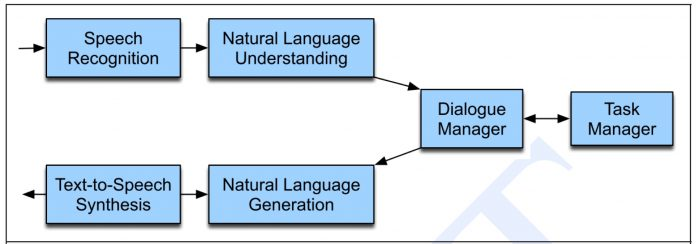
\includegraphics[width=10cm]{images/k.jpg}
    \caption{Kiến trúc cơ bản của một hệ thống giao tiếp tự động}
    \label{fig:system-class-intent}
\end{figure}

Các hệ thống chatbot giao tiếp với con người bằng giọng nói (như Siri) hoặc bằng văn bản (như các chatbot phát triển trên nền Facebook Messenger). Dù giao tiếp bằng hình thức nào, chatbot cũng cần phải hiểu văn bản để có thể đưa ra những câu trả lời phù hợp cho khách hàng. Thành phần đảm nhiệm công việc này trong hệ thống chatbot được gọi là \ac{nlu}, trong đó có rất nhiều các kỹ thuật xử lý ngôn ngữ tự nhiên (\ac{nlp}) được áp dụng.
\\
Hai thành phần liên quan đến xử lý ngôn ngữ tự nhiên không thể thiếu của một \ac{nlu} module là bộ phân loại ý định và nhận diện thực thể (NER). Phân loại ý định giúp chat-bot hiểu ý định của người dùng. Về mặt bản chất phân loại ý định chính là một bài toán phân loại câu với tập nhãn là các ý định có thể có của người dùng (đã được định nghĩa từ trước). NER giúp chat-bot trích xuất các thông tin trong yêu cầu/câu trả lời của người dùng. Các thông tin đó có thể là tên sản phẩm, địa chỉ, số điện thoại, số tài khoản của người dùng,… NER là một bài toán gán nhãn chuỗi cơ bản: cho vào một câu đầu vào, trích xuất tất cả các thực thể định danh trong câu và phân loại chúng vào một trong các nhãn đã được định nghĩa từ trước.
\\
Một thành phần xử lý ngôn ngữ tự nhiên khác có thể được thêm vào chat-bot là bộ quản lý hội thoại, bộ sinh ngôn ngữ (NLG), và bộ phân tích cảm xúc. Một bộ quản lý hội thoại sẽ lưu trữ, phân tích và tận dụng ngữ cảnh cuộc hội thoại và giúp chat-bot suy luận hành động tiếp theo trong khi NLG giúp sinh câu trả lời đầy đủ, tự nhiên nhất bằng ngôn ngữ tự nhiên cho chat-bot. Một bộ phân tích cảm xúc có thể cần bởi vì cùng một câu có thể mang nhiều nghĩa khác nhau trong các văn cảnh khác nhau, do đó có thể cần được trả lời theo các cách khác nhau phụ thuộc vào cảm xúc của người dùng.
\\
Bài luận này chủ yếu nghiên cứu về phát hiện ý định và trích xuất thực thể trong NLU module.

\section{Các hệ thống tương tự}

Hiện nay, việc xây dựng chatbot trong nhiều lĩnh vực như kinh doanh, y tế, giải trí,... khá là phát triển và đem lại được nhiều lợi ích lớn đối với người dùng. Trong lĩnh vực chỉ đường, chúng em nhận thấy rằng hiện chưa có chatbot nào được xây dựng, nhưng cũng có không ít các ứng dụng dùng để chỉ đường như Google Maps\cite{ggmaps},...

Google Maps là một dịch vụ bản đồ web được phát triển bởi Google. Nó cung cấp hình ảnh vệ tinh, chụp ảnh trên không, bản đồ đường phố, chế độ xem toàn cảnh tương tác 360° của đường phố, điều kiện giao thông thời gian thực và lập kế hoạch tuyến đường để đi bộ, xe hơi, xe đạp và máy bay hoặc giao thông công cộng. Năm 2020, Google Maps được sử dụng bởi hơn 1 tỷ người mỗi tháng trên thế giới.

Google Maps khởi đầu được thiết kế bởi hai anh em người Đan Mạch, tại công ty Where 2 Technologies có trụ sở tại Sydney. Lần đầu tiên nó được thiết kế để người dùng tải xuống riêng biệt, nhưng sau đó công ty đã trình bày ý tưởng về một sản phẩm hoàn toàn dựa trên Web cho ban quản lý của Google, thay đổi phương thức phân phối. Vào tháng 10 năm 2004, công ty được mua lại bởi Google - nơi nó chuyển thành ứng dụng web Google Maps. Sản phẩm hiện đã xuất hiện ở cả hai phiên bản web và mobile.

Google Map hiện giờ rất phố biến đối với người dùng và nó có rất nhiều tính năng về vị trí, trong đó có thể nói tính năng chỉ dẫn đường đi là vô cùng phổ biến với người dùng.

Tính năng chỉ đường của Google Maps cung cấp công cụ lập kế hoạch tuyến đường, cho phép người dùng tìm chỉ đường khả dụng thông qua lái xe, giao thông công cộng, đi bộ hoặc đi xe đạp.

Ứng dụng Google Maps trên điện thoại cũng tích hợp sử dụng thu âm, chuyển giọng nói thành văn bản khi nhập điểm bắt đầu và điểm kết thúc để người dùng có thể dễ nhập điểm đầu và cuối.

\begin{figure}[H]
    \centering
    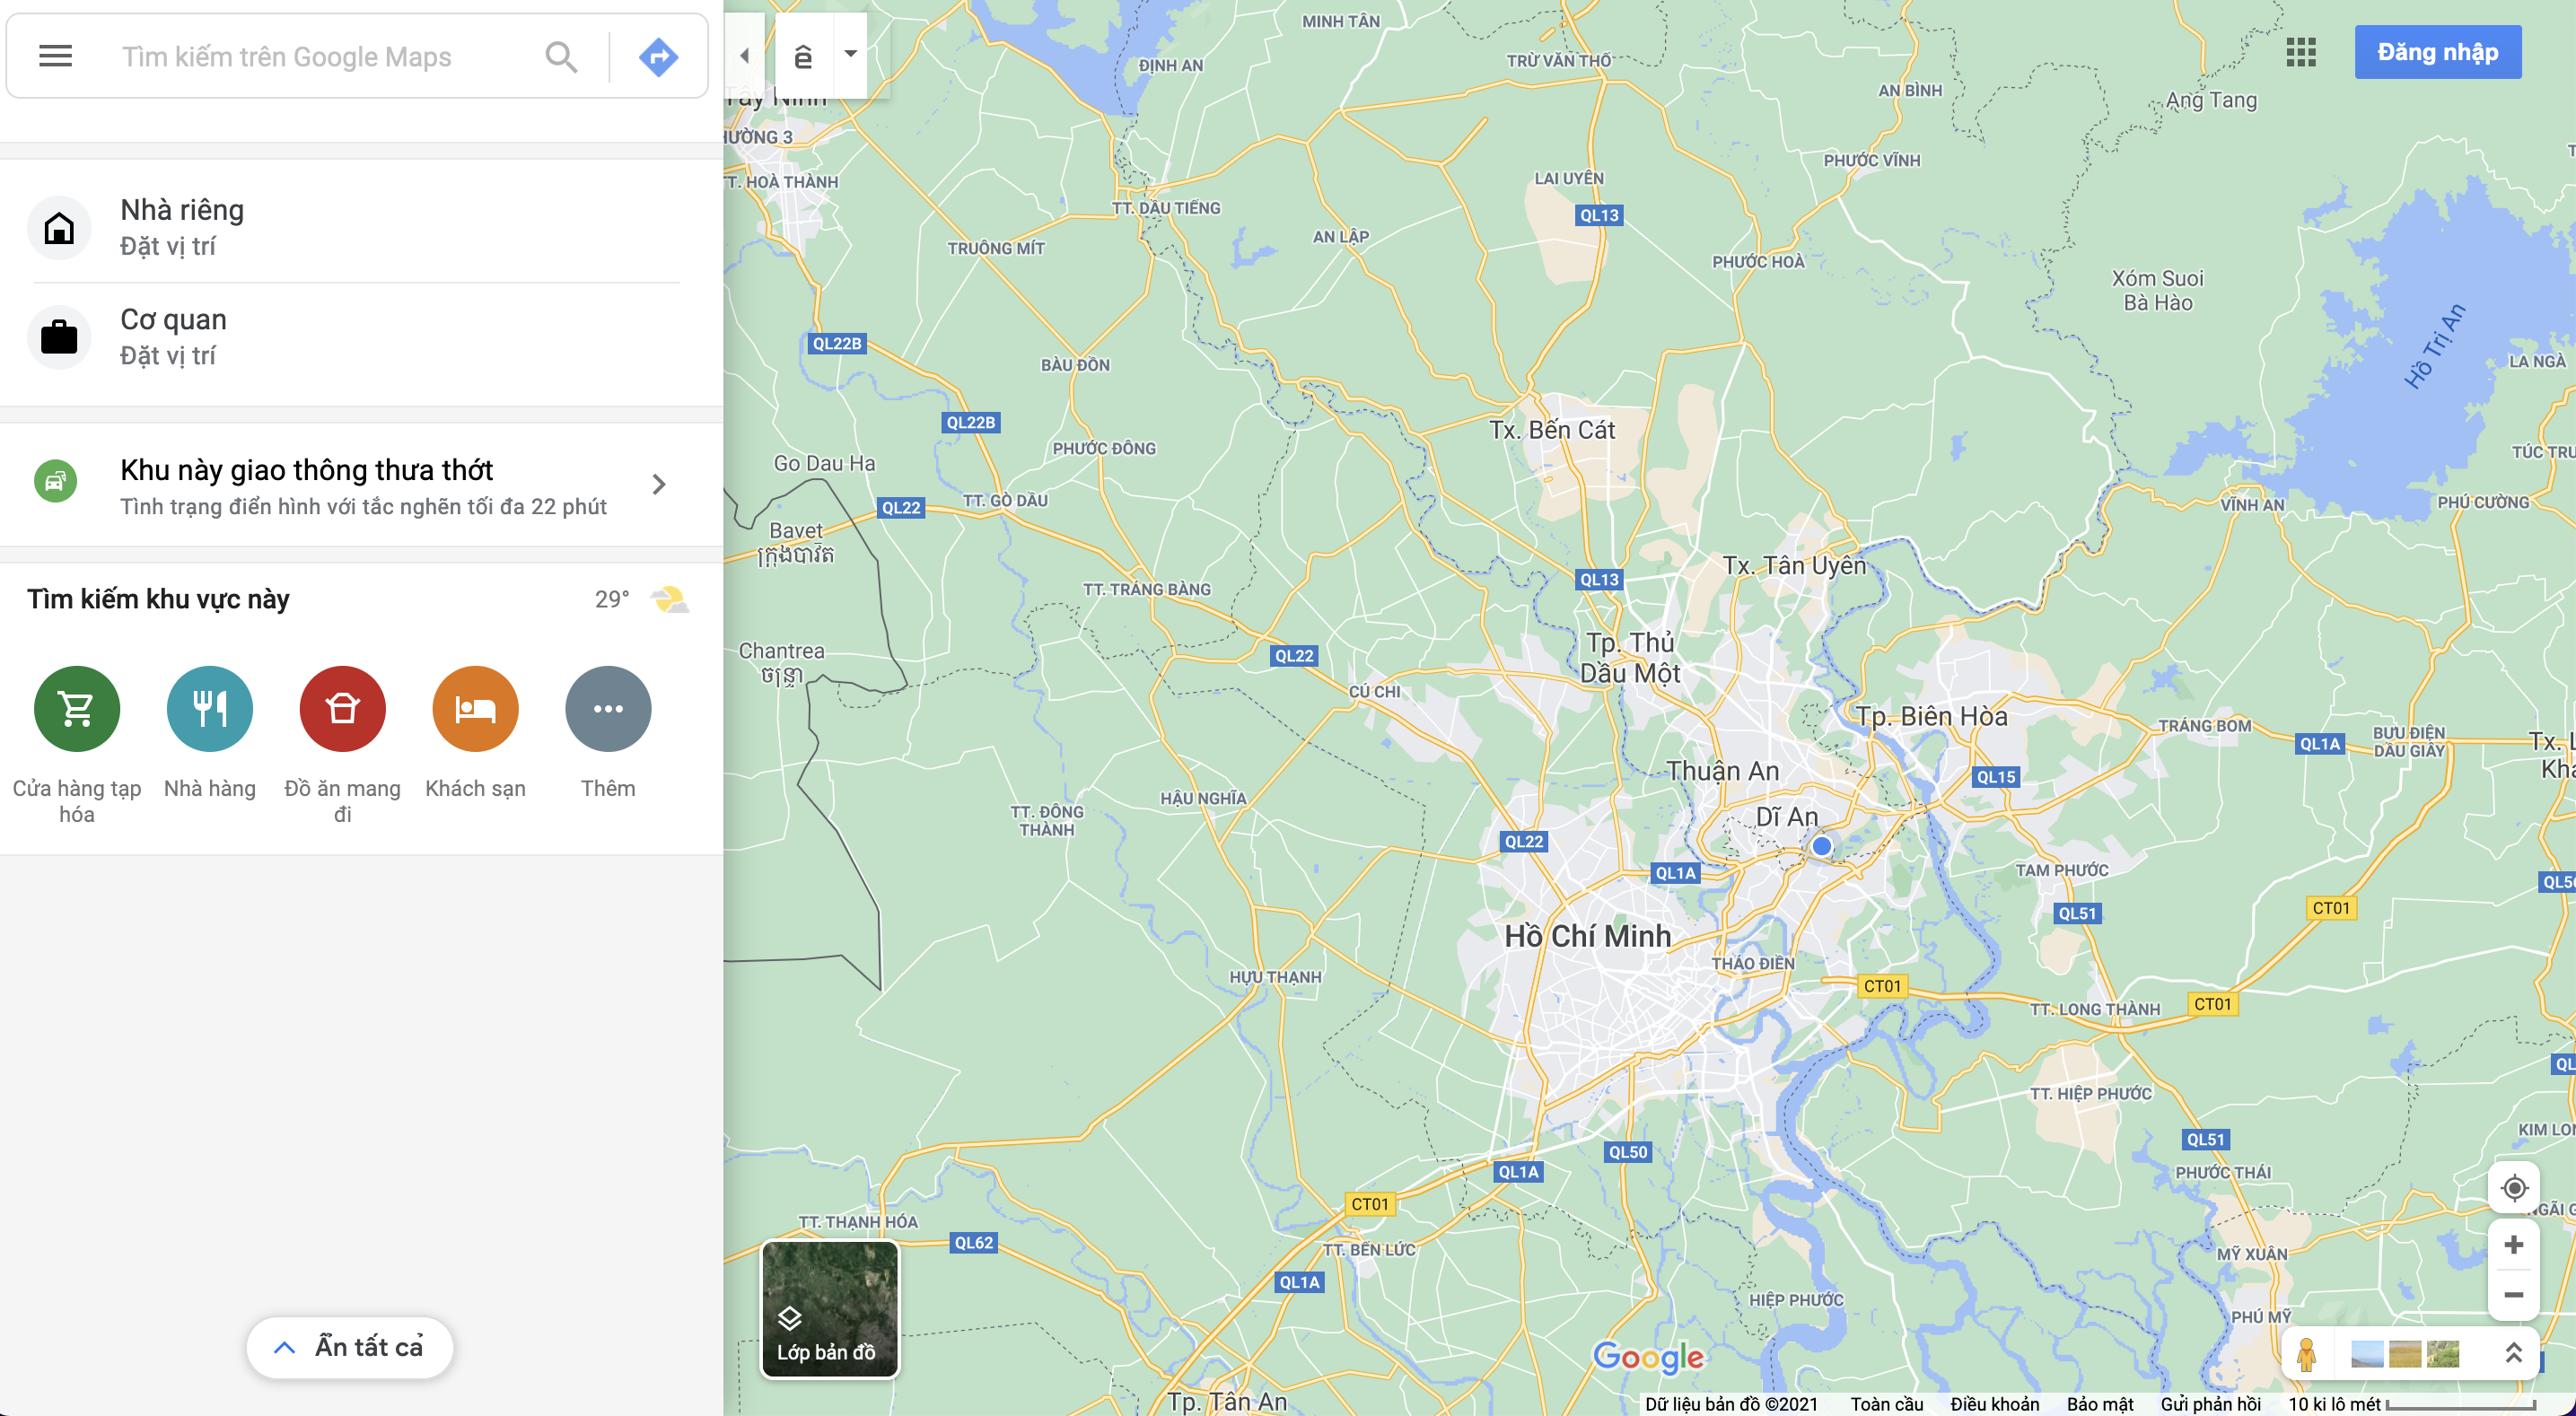
\includegraphics[width=10cm]{images/HomePage-GoogleMaps.png}
    \caption{Trang chủ Google Maps}
    \label{fig:homepage-ggmaps}
\end{figure}

Android Auto là một ứng dụng di động được phát triển bởi Google nhằm đưa các tính năng từ một thiết bị Android (ví dụ như điện thoại thông minh) lên hệ thống bảng thông báo và giải trí tương thích trên xe hơi.

\begin{figure}[H]
    \centering
    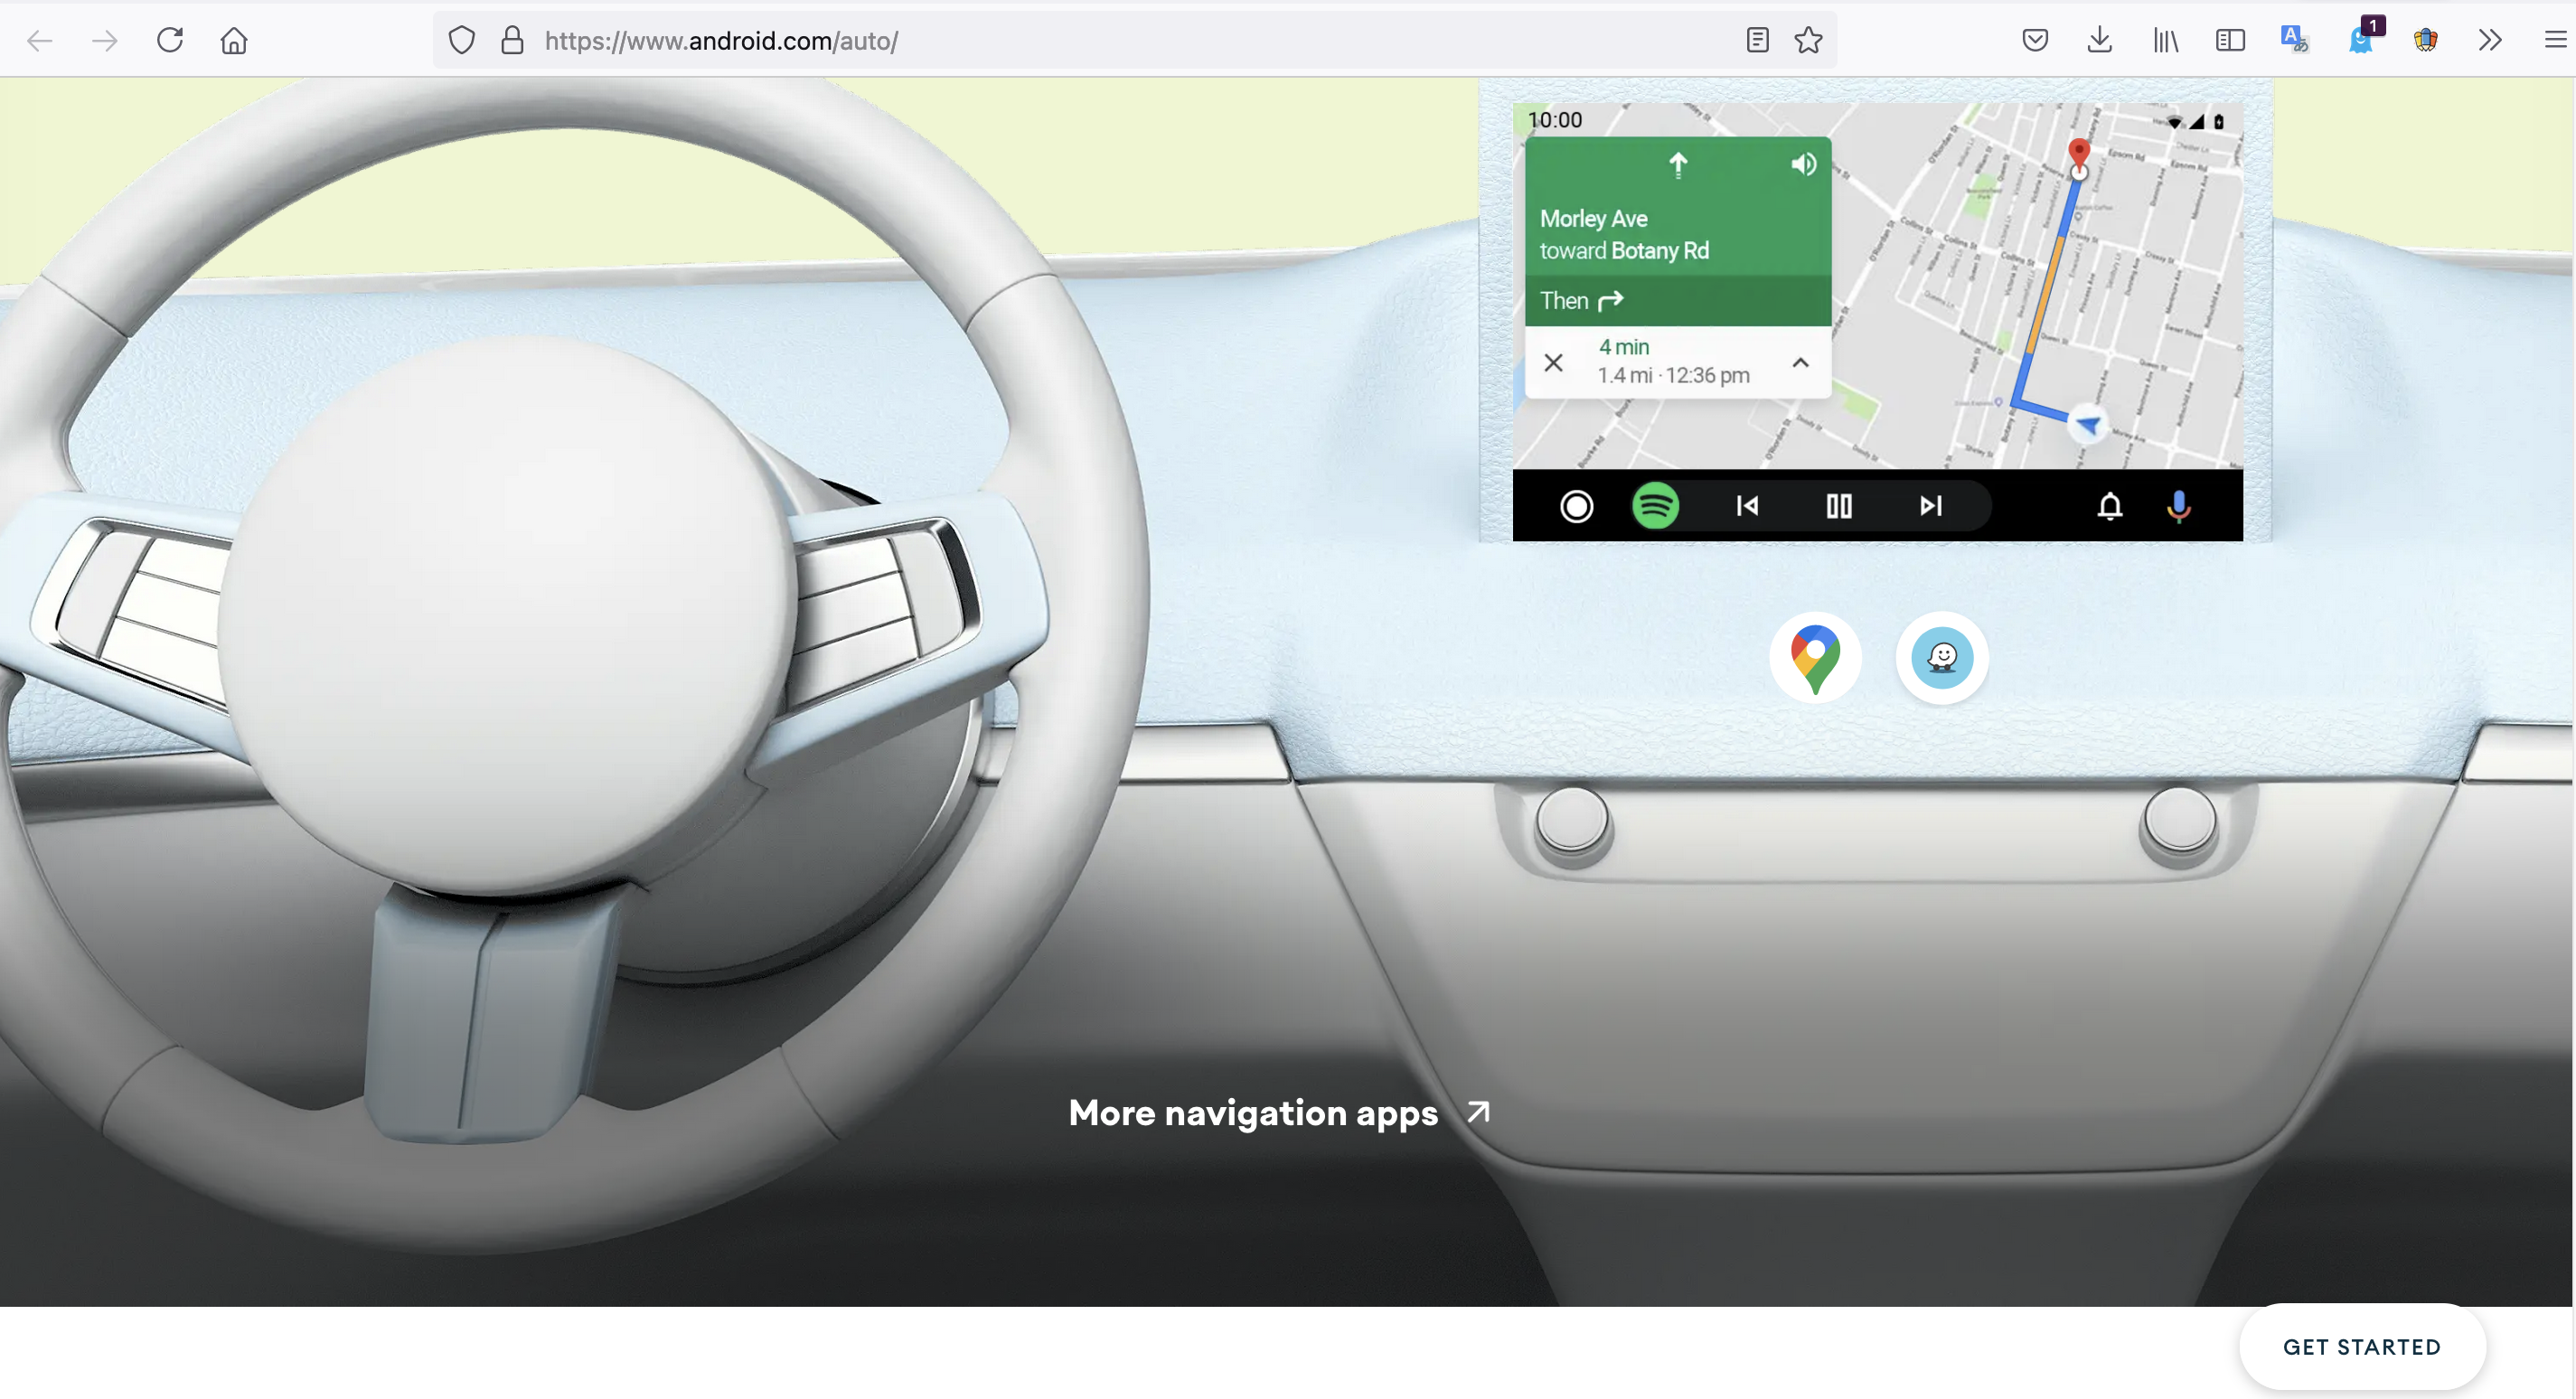
\includegraphics[width=10cm]{images/Android-Auto.png}
    \caption{Trang chủ Android Auto}
    \label{fig:homepage-android-auto}
\end{figure}

Kết nối điện thoại với màn hình ô tô — ứng dụng Android sẽ hiển thị trên màn hình hiển thị của xe. Nhấn để nhận chỉ đường lái xe hoặc nói chuyện để gửi tin nhắn. Thậm chí gọi điện thoại rảnh tay cho mẹ bạn. Android Auto được tạo ra để giúp bạn tập trung vào đường đi. Và vui vẻ trên đường đi. Chỉ cần cắm vào và đi.

\begin{figure}[H]
    \centering
    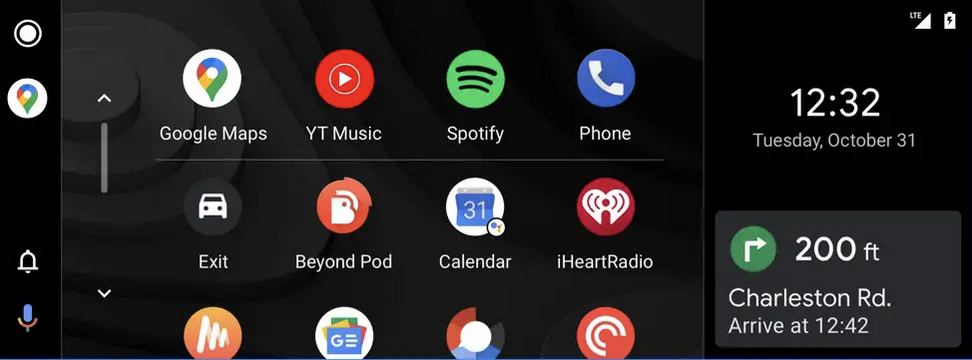
\includegraphics[width=10cm]{images/widescreen.png}
    \caption{Xem mọi thứ trên màn hình rộng.}
    \label{fig:homepage-widescreen-Android}
\end{figure}

Với mong muốn xây dựng một ứng dụng chatbot sử dụng trong lĩnh vực chỉ đường, chúng em xây dựng một ứng dụng tiếng Việt, trong đó có sử dụng giọng nói để tương tác với ứng dụng, hỏi đường chỉ bằng một câu nói dễ dàng, sử dụng được mọi lúc, một cách đơn giản mà không làm mất đi sự tập trung của người dùng khi lái xe.

\section{Một số phương pháp hiểu ngôn ngữ tự nhiên}

\begin{itemize}
    \item Rasa \ac{nlu}
          \begin{figure}[htp]
              \centering
              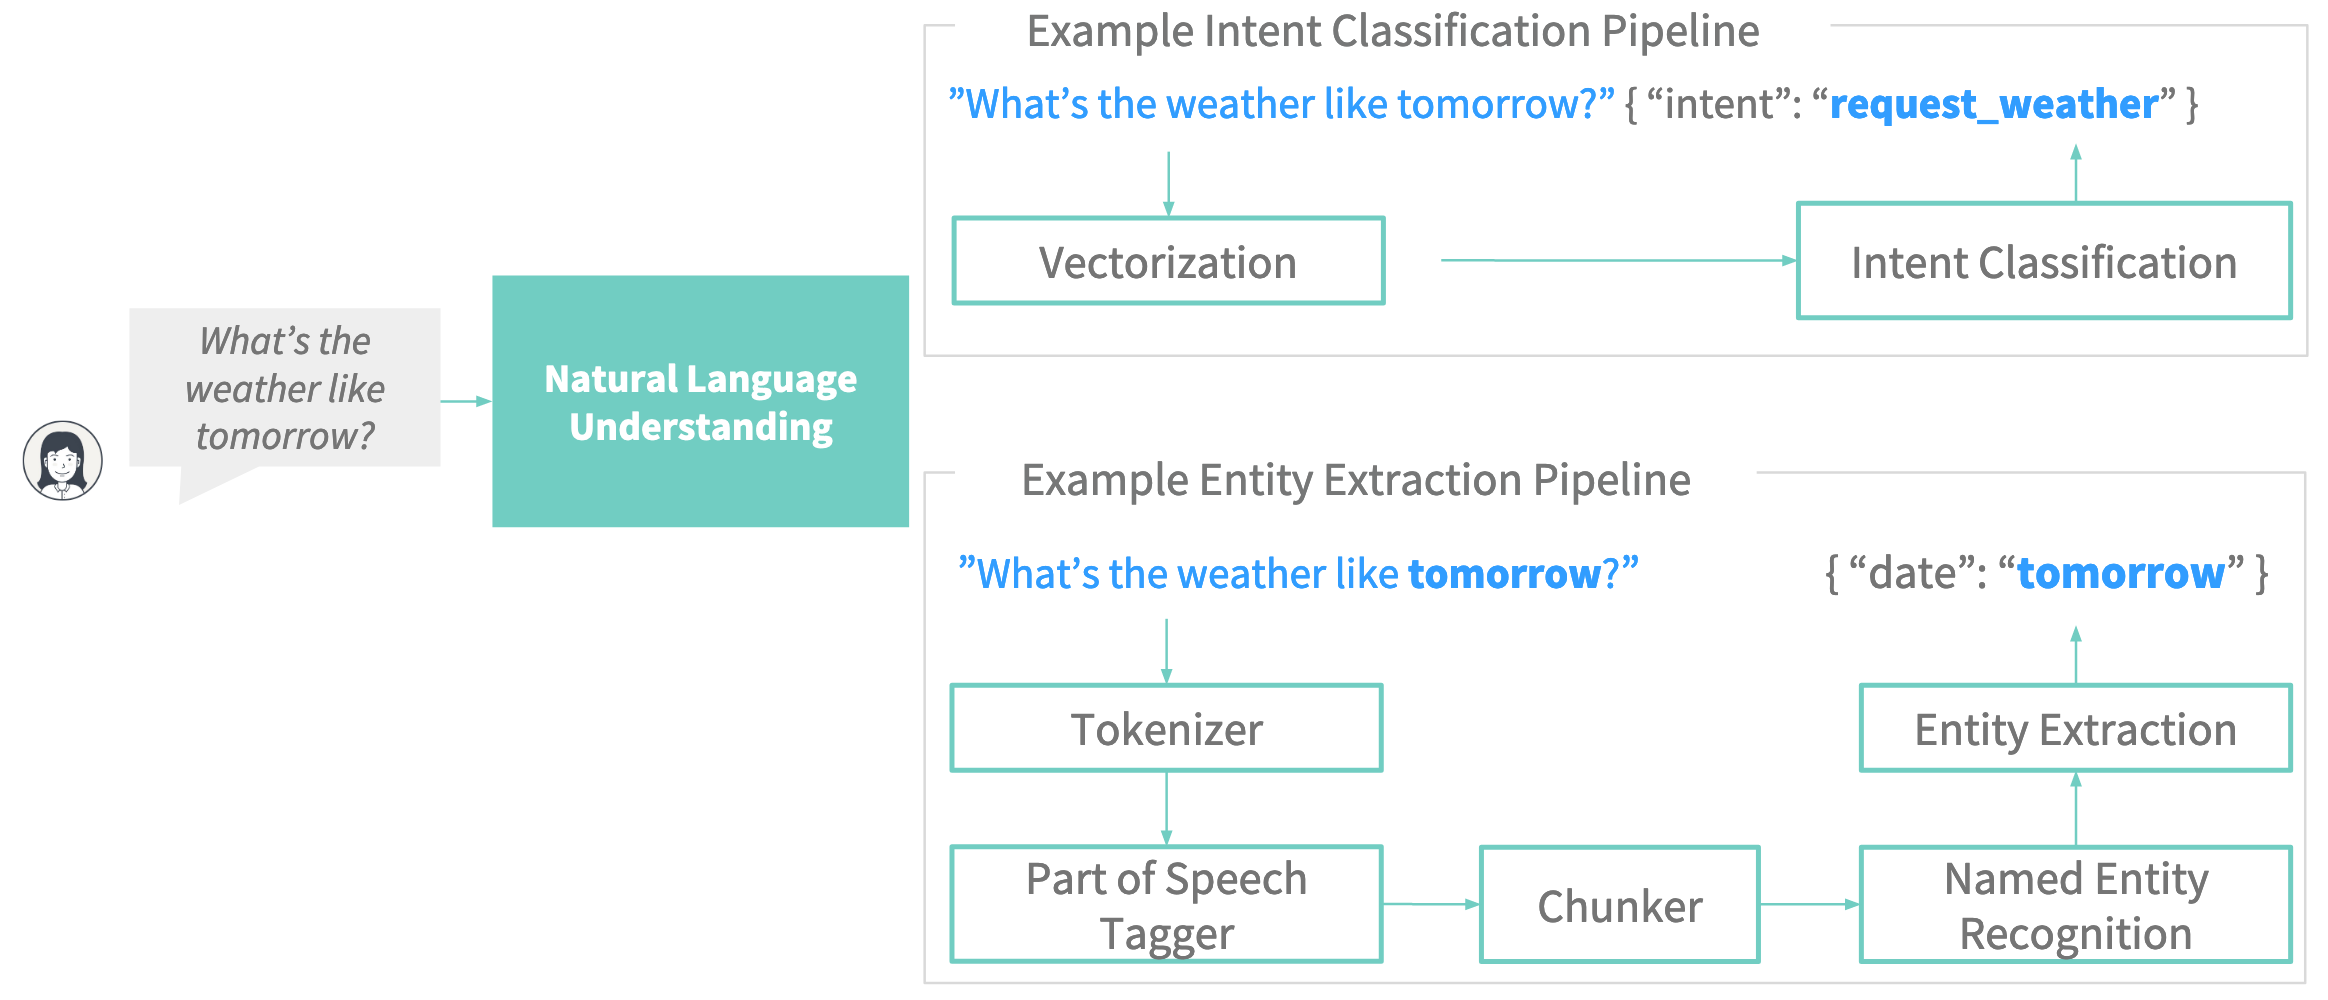
\includegraphics[width=10cm]{images/Rasa-NLU.png}
              \caption{Sơ đồ hệ thống Rasa-\ac{nlu}}
              \label{fig:rasa-nlu}
          \end{figure}
    \item Snips \ac{nlu}
          \begin{figure}[htp]
              \centering
              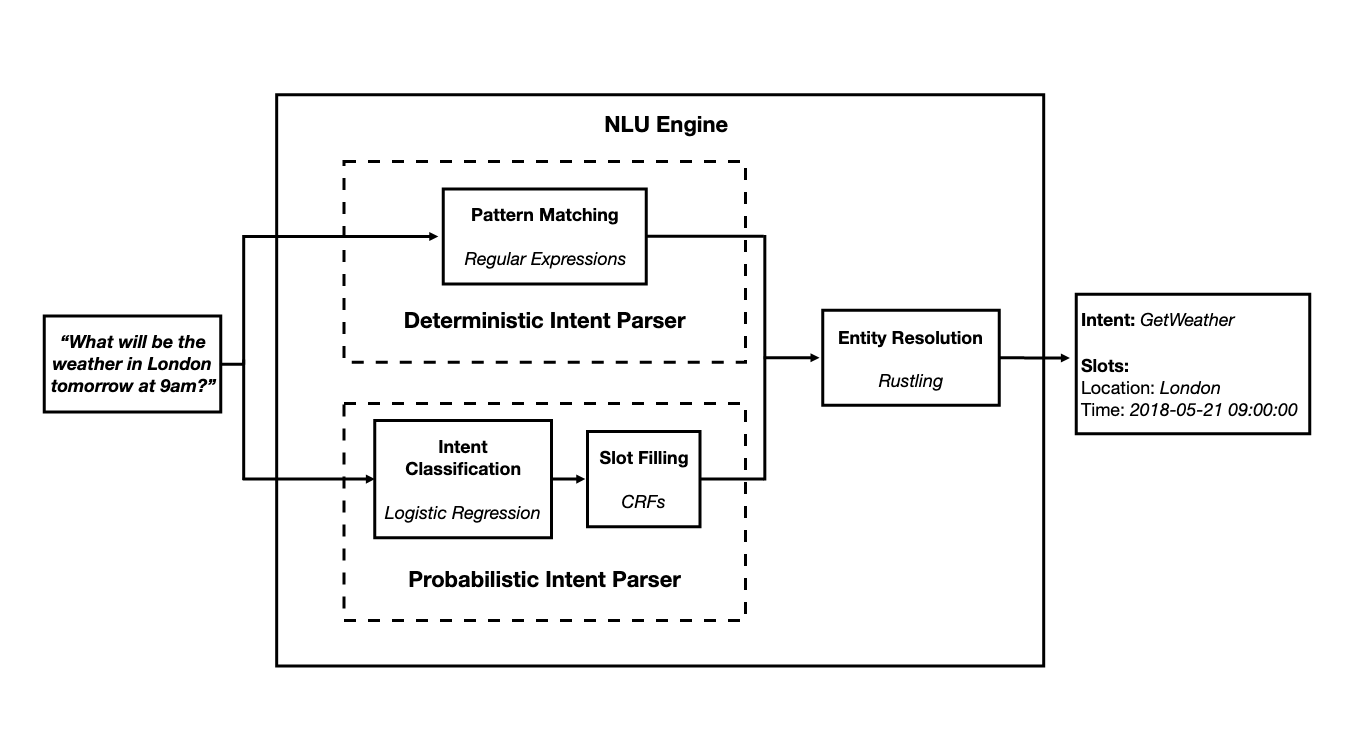
\includegraphics[width=10cm]{images/Snips-NLU.png}
              \caption{Sơ đồ hệ thống Snips-\ac{nlu}}
              \label{fig:snips-nlu}
          \end{figure}
          Có thể khái quát các luồng xử lý của snips-NLU \cite{snips-nlu} như sau:
          Hệ thống Snips-NLU (hình \ref{fig:snips-nlu}) chứa một thành phần chính, NLU Engine, bản thân nó bao gồm một số thành phần sau:
          \begin{itemize}
              \item Deterministic intent parser: Mục tiêu của trình phân tích cú pháp xác định là cung cấp độ mạnh mẽ và trải nghiệm có thể dự đoán được cho người dùng vì nó được đảm bảo đạt được 1.0 F1-Score trên các ví dụ đào tạo. Các truy vấn có trong dữ liệu huấn luyện được sử dụng để xây dựng các mẫu bao gồm tất cả các tổ hợp giá trị thực thể.
              \item Probabilistic intent parser: Trình phân tích cú pháp mục đích nhằm mục đích mở rộng phân tích cú pháp vượt ra ngoài các ví dụ đào tạo và nhận ra các biến thể không xuất hiện trong dữ liệu đào tạo. Nó cung cấp sức mạnh tổng quát hóa mà trình phân tích cú pháp xác định thiếu. Thông qua hai bước intent classification (xác định ý định) and slot filling (trích xuất thực thể).
              \item Entity resolution:
          \end{itemize}
\end{itemize}
\section{So sánh các nền tảng hiểu ngôn ngữ tự nhiên}

\begin{itemize}
    \item[--] 	Hầu hết các chatbot và trợ lý giọng nói đều dựa vào các dịch vụ đám mây cho NLU của họ. Những dịch vụ phổ biến nhất bao gồm Dialogflow\footnote{\url{https://dialogflow.com/}}(Google, ex API.ai), Amazon Lex\footnote{\url{https://docs.aws.amazon.com/lex/latest/dg/what-is.html}}, Amazon Alexa\footnote{\url{https://developer.amazon.com/docs/ask-overviews/build-skills-with-the-alexa-skills-kit.html}}, Luis.ai\footnote{\url{https://www.luis.ai/}} (Microsoft), Wit.ai\footnote{\url{https://wit.ai/}} (Facebook) và IBM Watson\footnote{\url{https://www.ibm.com/watson/services/natural-language-understanding/}}.
    \item[--] Một điểm chung của tất cả các giải pháp này là chúng hoàn toàn tập trung, chạy trên máy chủ của nhà cung cấp. Điều này có nghĩa là họ có thể truy cập tất cả dữ liệu đang được gửi đến dịch vụ của họ và sử dụng lại nó theo ý muốn.
    \item[--] Snips NLU\footnote{\url{https://github.com/snipsco/snips-nlu}} là một thư viện Python có thể được sử dụng để dễ dàng đào tạo các mô hình và sử dụng các mô hình được đào tạo để đưa ra dự đoán về các truy vấn mới.

    \item[--] Snips NLU là mã nguồn mở, chạy offline nên không bao giờ đụng vào, xử lý hoặc thu thập bất kỳ dữ liệu người dùng nào.

    \item[--] Ngoài ra, chúng ta còn có Snips NLU-rs\footnote{\url{https://github.com/snipsco/snips-nlu-rs}}, một triển khai Rust tập trung vào phần dự đoán (hay còn gọi là suy luận). Thư viện này có thể được sử dụng trên hầu hết các kiến trúc hiện đại: trên các thiết bị nhỏ được kết nối, trên thiết bị di động, trên máy tính để bàn hoặc trên máy chủ. Nó hiện có thể xử lý 5 ngôn ngữ (tiếng Anh, tiếng Pháp, tiếng Đức, tiếng Tây Ban Nha và tiếng Hàn), với nhiều ngôn ngữ được bổ sung thường xuyên.
    \item[--] Bây giờ chúng ta hãy xem xét tốc độ của Snips NLU , chúng ta sẽ tập trung vào hiệu suất và độ chính xác, cho thấy rằng công nghệ này hoạt động ngang bằng hoặc tốt hơn các giải pháp dựa trên đám mây.

        \textbf{Thời gian chạy suy luận}

    \item[--] Đây là thời gian chạy trung bình để xử lý một truy vấn trong một trợ lý điển hình\footnote{\url{https://github.com/sebischair/NLU-Evaluation-Corpora/blob/master/AskUbuntuCorpus.json}}:

        \begin{figure}[htp]
            \centering
            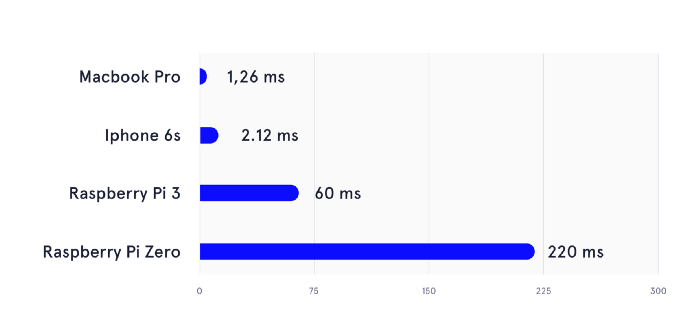
\includegraphics[width=10cm]{images/ComparisonOfNLU/averageTime.png}
            \caption{Average time to parse a query with Snips NLU-rs}
            \label{fig:system-class-intent}
        \end{figure}

        \item[--]Trung bình, mất chưa đến 2 mili giây để phân tích cú pháp một truy vấn trên Macbook Pro 2015 với Core i7 2,5 GHz. Vì nền tảng được tối ưu hóa cho hiệu suất và không yêu cầu quyền truy cập mạng, nên thời gian thu được thông thường có thể nhanh gấp 2 lần so với việc sử dụng dịch vụ đám mây!

        \item[--]Bộ nhớ cũng đã được tối ưu hóa, từ vài trăm KB RAM cho các trường hợp thông thường đến vài MB cho các trợ lý phức tạp nhất. Điều đó cũng có nghĩa là các máy chủ mạnh hơn có thể xử lý hàng trăm trường hợp song song.

        \textbf{Sự chính xác}

        \item[--]Để xác minh rằng công cụ Snips NLU hoạt động tốt, đội ngũ Snips đã so sánh\footnote{\url{https://medium.com/snips-ai/benchmarking-natural-language-understanding-systems-google-facebook-microsoft-and-snips-2b8ddcf9fb19}} nó với các dịch vụ đám mây, bao gồm API.ai (nay là DialogFlow, Google), Wit.ai (Facebook), Luis.ai (Microsoft) và Amazon Alexa. Mọi giải pháp đều được đào tạo bằng cách sử dụng cùng một bộ dữ liệu\footnote{\url{https://github.com/snipsco/nlu-benchmark/tree/master/2017-06-custom-intent-engines}} và được thử nghiệm trên cùng một bộ thử nghiệm. Kết quả cho thấy Snips NLU chính xác bằng hoặc tốt hơn các giải pháp đám mây ở các nhiệm vụ khai thác vị trí, bất kể lượng dữ liệu đào tạo được sử dụng nhiều hay ít.

        \item[--]Bộ dữ liệu chứa 2400 truy vấn cho từng ý định, gồm 7 ý định:

        \begin{figure}[htp]
            \centering
            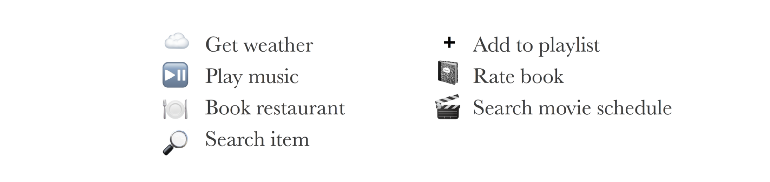
\includegraphics[width=10cm]{images/ComparisonOfNLU/7ntents.png}
            \caption{7 intents covered in this benchmark}
            \label{fig:system-class-intent}
        \end{figure}
        Bộ dữ liệu này có sẵn miễn phí trên Github\footnote{\url{https://github.com/snipsco/nlu-benchmark}}.
        \item[--]Với mọi hệ thống NLU, việc xây dựng mô hình luôn đi qua các bước giống nhau: nhập các ví dụ về các truy vấn có thể mà người dùng sẽ thực hiện và gắn thẻ các phân đoạn câu phù hợp với các thuộc tính mà bạn đang tìm kiếm.

        \item[--]Đội ngũ Snips đã tính toán hiệu suất của từng dịch vụ. Điều này được thực hiện bằng cách chọn ngẫu nhiên nhiều bộ đào tạo gồm 70 truy vấn cho mỗi mục đích nhất định, sau đó cung cấp cho từng NLU engine. Các hiệu suất được tính toán bằng cách đo lường hiệu suất trên một tập dữ liệu xác thực. Đối với mỗi ý định, đội ngũ Snips tính trung bình điểm số thu được qua nhiều lần lặp lại thử nghiệm. Chi tiết của quy trình được mô tả trên Github\footnote{\url{https://github.com/snipsco/nlu-benchmark}}. Dưới đây là kết quả thu được:

        \begin{figure}[htp]
            \centering
            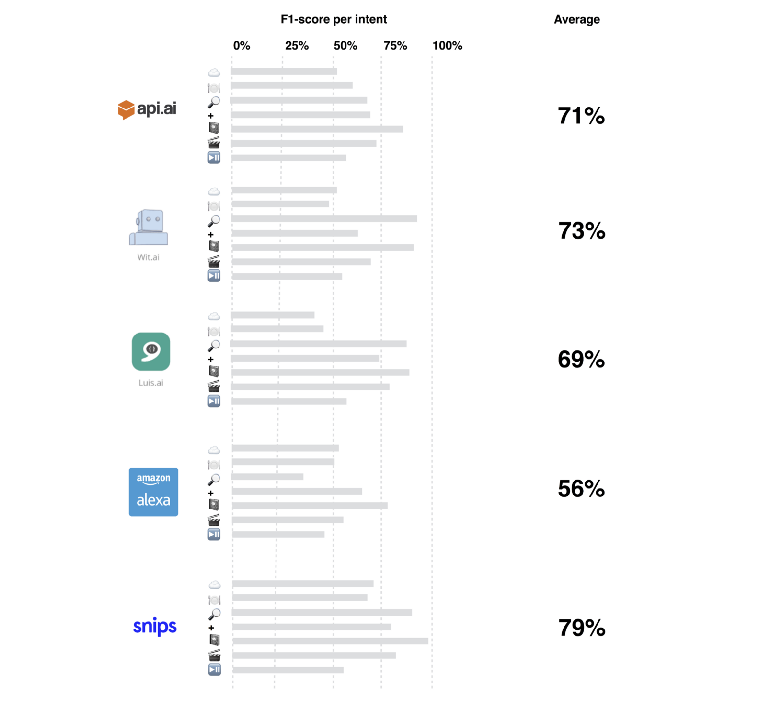
\includegraphics[width=10cm]{images/ComparisonOfNLU/f1Score70Intents.png}
            \caption{F1-score (per intent, and averaged) for the different providers trained on 70 queries / intent.}
            \label{fig:system-class-intent}
        \end{figure}

        \item[--]Những kết quả này cho thấy rằng công cụ NLU mà bạn tạo bằng Snips sẽ đáng tin cậy hơn đáng kể so với những gì đạt được với các nền tảng khác. Nếu chúng ta đi sâu vào chi tiết một chút, chúng ta thấy rằng các giải pháp của Microsoft, Facebook và Amazon bị thấp do độ nhạy kém của chúng: recall lần lượt là 53%, 56% và 49%, so với 65% đối với Google và 77% đối với Snips.

        \textbf{Một AI thực sự đáng tin cậy}

        \item[--]Điểm đáng chú ý chính là các hiệu suất đạt được trong bối cảnh này không hoàn hảo. Không có giải pháp nào trong số các giải pháp này đạt hơn 80%.

        \item[--]Có một lý do cho điều đó: thật khó để xử lý bất kỳ trường hợp nào có thể xảy ra, khi bạn chỉ thấy 70 ví dụ về một mục đích nhất định.

        \item[--]Nếu công cụ Snips NLU được đào tạo trên 2000 truy vấn thay vì 70, thì hiệu suất sẽ đạt được như sau:

        \begin{figure}[htp]
            \centering
            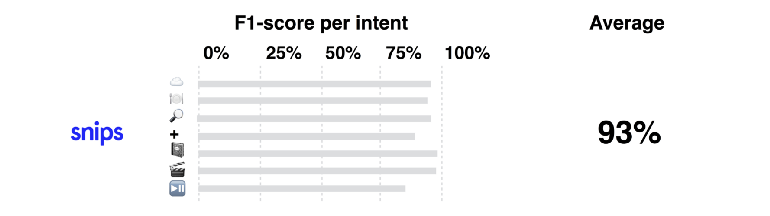
\includegraphics[width=10cm]{images/ComparisonOfNLU/f1Score2000Intents.png}
            \caption{F1-score (per intent, and averaged) for the Snips NLU engine trained on 2000 queries / intent.}
            \label{fig:system-class-intent}
        \end{figure}


        \item[--]Sau khi tăng dữ liệu đào tạo trên 2000 truy vấn trên mỗi mục đích, F1-score trung bình đã đạt 93%. Bên cạnh đó, các thuộc tính được trích xuất chính xác trong 95% trường hợp (precision) và khả năng xác định thuộc tính (recall) là hơn 90%.

        \item[--]Bằng hình ảnh minh họa cụ thể, hãy xem ba truy vấn được lấy từ bộ xác thực, để hiểu cách các giải pháp khác nhau hoạt động. Trong ví dụ đơn giản sau, tất cả các công cụ NLU hoạt động chính xác:

        \begin{figure}[htp]
            \centering
            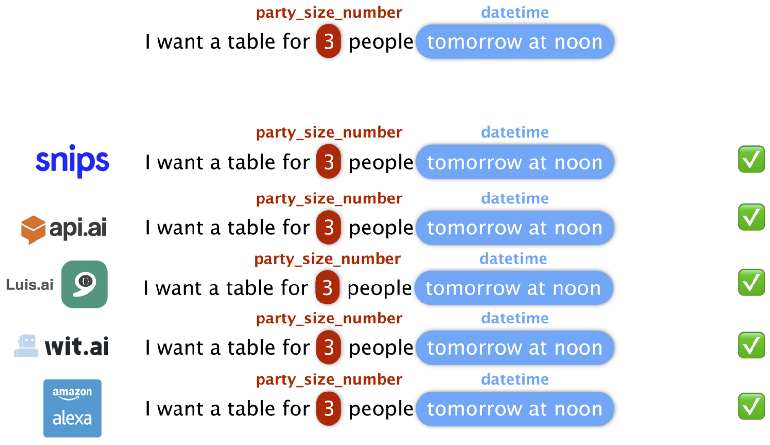
\includegraphics[width=10cm]{images/ComparisonOfNLU/slotfilling1.png}

            \label{fig:system-class-intent}
        \end{figure}

        \item[--]Ở dưới đây, Alexa nhầm lẫn Sacaton với một quốc gia và với ngày giờ bởi API.ai. API.ai cùng với Wit và Alexa hiểu rằng gluten là một loại nhà hàng. Mặt khác, Luis không phát hiện ra bất kỳ thuộc tính nào.

        \begin{figure}[htp]
            \centering
            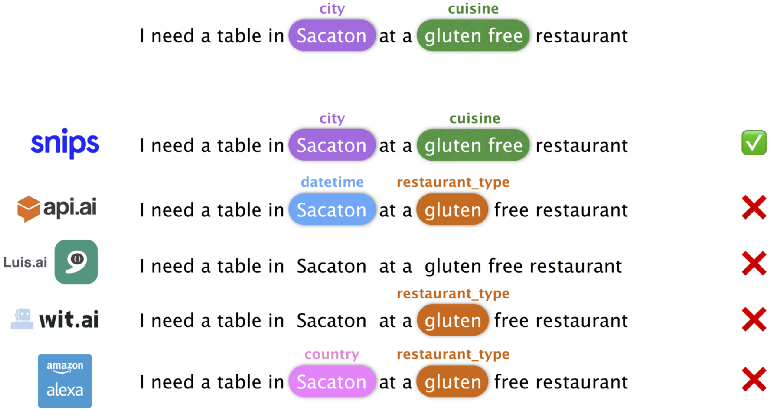
\includegraphics[width=10cm]{images/ComparisonOfNLU/slotfilling2.png}

            \label{fig:system-class-intent}
        \end{figure}

        \item[--]Trong ví dụ cuối cùng này, chúng ta thấy rằng một lần nữa, Luis không phát hiện ra bất kỳ vị trí nào. API.ai nhầm lẫn the best bistro với tên nhà hàng và Wit.ai diễn giải đại từ “me” là trạng thái mà người dùng muốn đặt chỗ. Mặt khác, Alexa có câu trả lời chính xác.

        \begin{figure}[htp]
            \centering
            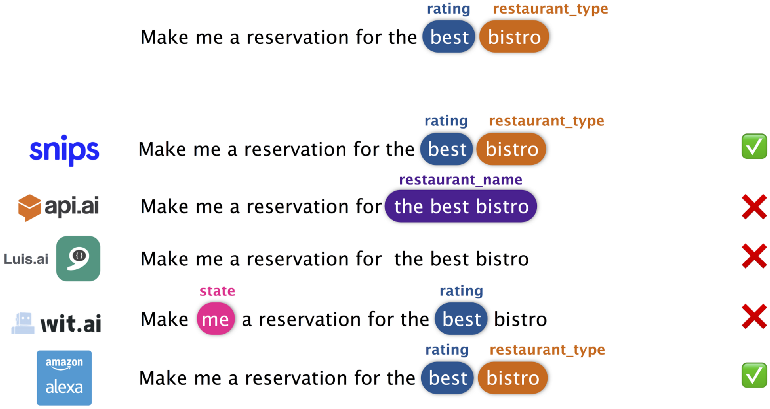
\includegraphics[width=10cm]{images/ComparisonOfNLU/slotfilling3.png}

            \label{fig:system-class-intent}
        \end{figure}


        \item[--]Dữ liệu điểm chuẩn, cũng như hiệu suất chi tiết của từng nhà cung cấp có thể được tìm thấy trên Github\footnote{\url{https://github.com/snipsco/nlu-benchmark}}.

        \begin{figure}[htp]
            \centering
            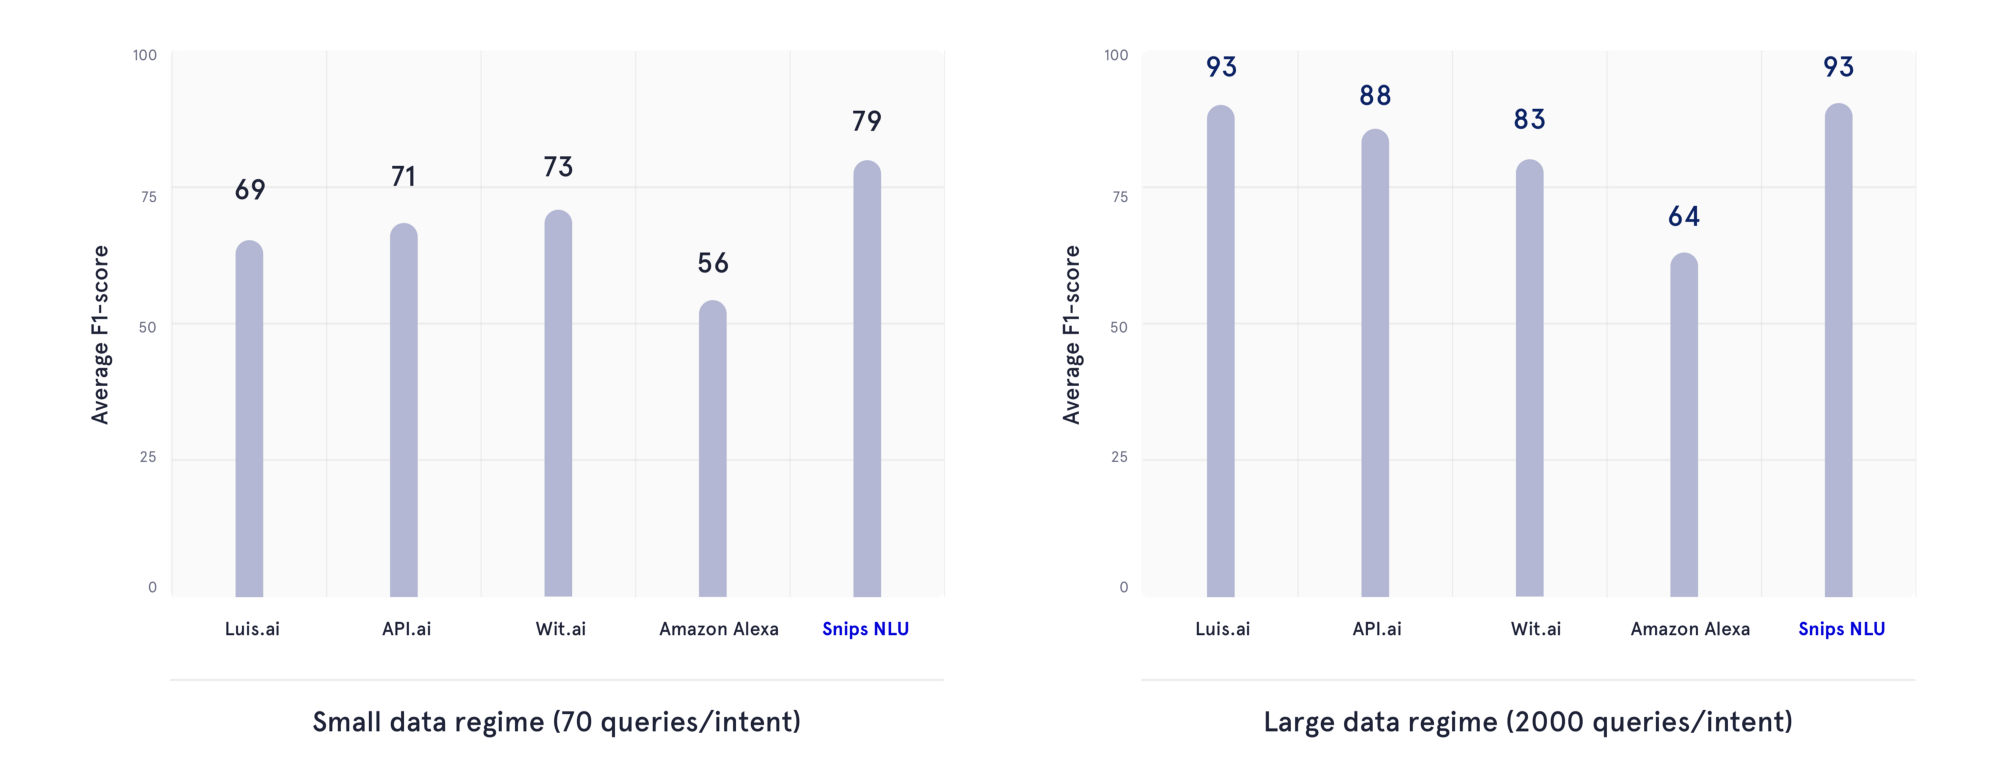
\includegraphics[width=10cm]{images/ComparisonOfNLU/benchmarking.png}
            \caption{Benchmarking Natural Language Understanding Systems}
            \label{fig:system-class-intent}
        \end{figure}

        \item[--]Đội ngũ Snips cũng tái sản xuất một điểm chuẩn\footnote{\url{http://workshop.colips.org/wochat/@sigdial2017/documents/SIGDIAL22.pdf}} được công bố vào mùa hè năm ngoái. Trong bài viết này, các tác giả đã đánh giá hiệu suất của API.ai (nay là Dialogflow, Google), Luis.ai (Microsoft), IBM Watson và Rasa NLU\footnote{\url{https://nlu.rasa.ai/}}. Để công bằng, đội ngũ Snips đã sử dụng phiên bản mới nhất của Rasa NLU và so sánh nó với phiên bản mới nhất của Snips NLU (cả hai đều có màu xanh lam đậm).

        \begin{figure}[htp]
            \centering
            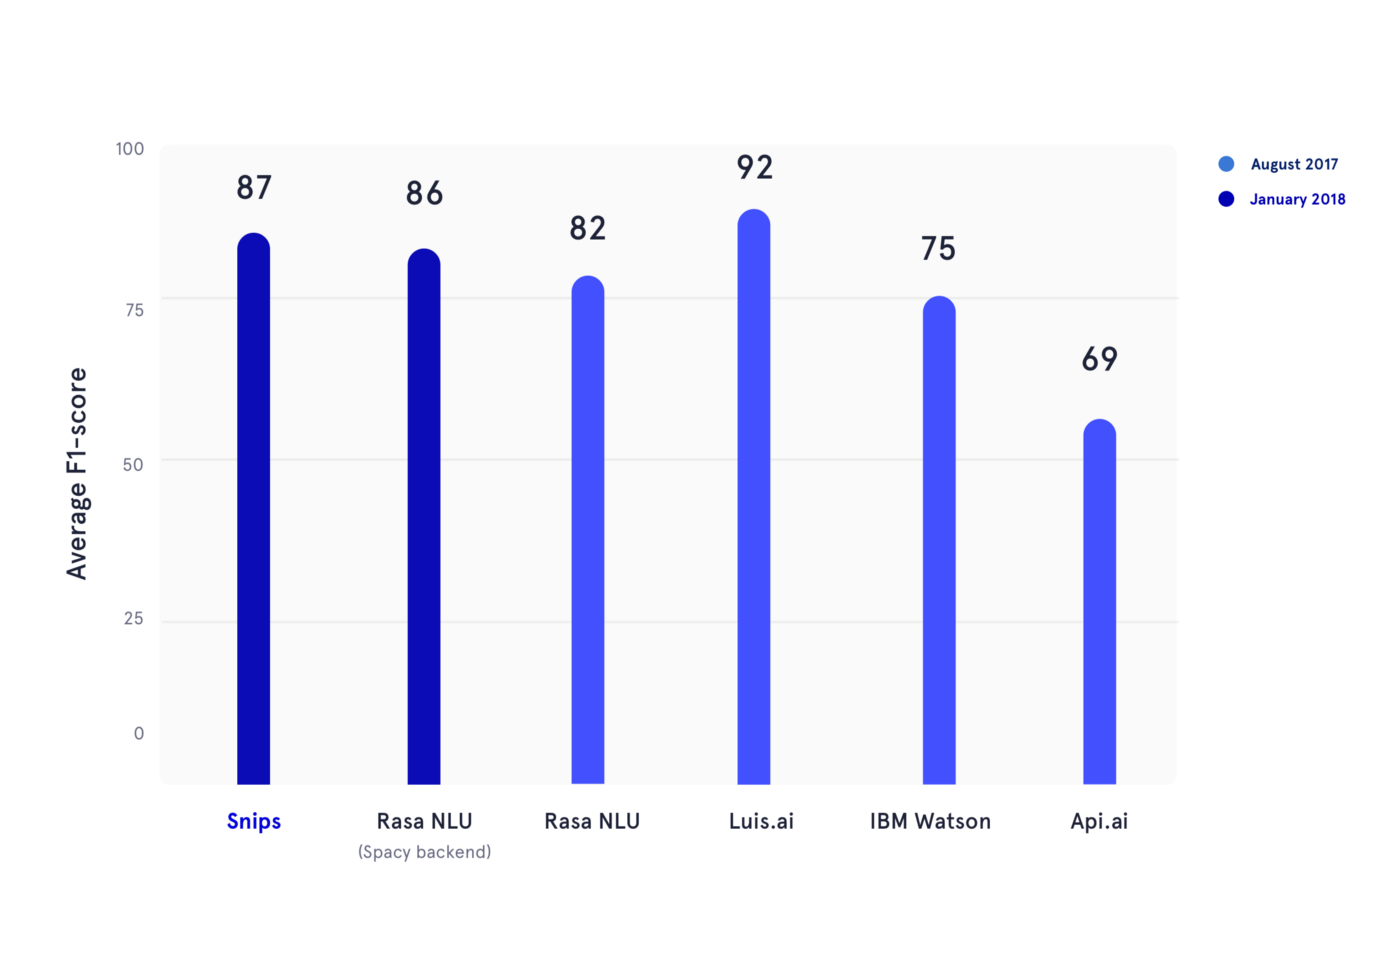
\includegraphics[width=10cm]{images/ComparisonOfNLU/Reproducing.png}
            \caption{Reproducing “Evaluating Natural Language Understanding Services for Conversational Question Answering Systems”.}
            \label{fig:system-class-intent}
        \end{figure}

        \item[--]Trên tất cả các điểm chuẩn, Snips NLU xếp hạng cao nhất hoặc cao thứ hai, mặc dù nhanh hơn và nhẹ hơn mọi giải pháp khác. Điều này cho thấy việc lựa chọn giải pháp NLU đám mây - và hy sinh quyền riêng tư và quyền kiểm soát dữ liệu - hoàn toàn không còn cần thiết nữa. Snips NLU là một giải pháp thay thế mạnh mẽ cho các giải pháp hiện có.



\end{itemize}